\documentclass[../slides.tex]{subfiles}

\title{Introducción a la Progamación Lineal}
\subtitle{Investigación de Operaciones} % 6 hours. 2 sessions
\AtBeginSection[] % Do nothing for \section* %
{
\begin{frame}<beamer> 
  \frametitle{Agenda}
  \tableofcontents[currentsection] 
\end{frame}
}

\begin{document}

\begin{frame}
  \maketitle
\end{frame}


     \begin{frame}{Agenda}
   \tableofcontents
 \end{frame}



\section{Estructura de los modelos matemáticos}
\label{sec:formulations}

\begin{frame}{Requerimientos}
  \begin{enumerate} \parskip2mm \justifying
  \item<only@1> Función objetivo bien definida para maximizar o minimizar (costo, utilidad, cantidades a producir, etc.) 
  \item<only@1> Restricciones sobre la función objetivo. Estas restricciones se deben expresar como ecuaciones o desigualdades en términos de las variables.
  \item<only@1> Deben existir alternativas de acción. Por ejemplo, un producto se puede fabricar en diferentes máquinas y se debe determinar la cantidad que se va a fabricar en cada una de ellas. 
  \item<only@2> Las variables de decisión deben estar relacionadas y ser no negativas. La condición de no negatividad nos indica que estamos trabajando con problemas reales por lo que cantidades negativas serían ilógicas.
  \item<only@2> Los recursos son escasos. Si una empresa fabrica grandes cantidades de un producto en particular, entonces sde deben fabricar cantidades menores de otros productos debido a que la capacidad de producción es limitada.
  \end{enumerate}
\end{frame}

\begin{frame}{Supuestos}
  \begin{enumerate} \parskip3mm \justifying
  \item<only@1> Proporcionalidad. Si la ganancia es de \$ 10 por unidad de un producto, entonces por producir 12 unidades de ese producto se obtiene una utilidad total de $10 \times 12 = 120.$ De manera similar, si un producto tarda 5 horas en ser procesado, entonces, producir 10 unidades de ese producto, consumirá un total de 50 horas. 
  \item<only@1> Aditividad. Si se consumen $t_1$ horas en máquina A para producir producto 1 y $t_2$ horas para producto 2, el tiempo total para los productos 1 y 2 en la máquina A será de $t_1 + t_2$ horas.
  \item<only@1> Continuidad. Los valores de las variables de decisión puden tomar valores continuos (racionales no negativos).
  \item<only@2> Certeza. Los valores de los parámetros, por ejemplo, los coeficientes en la función objetivo, coeficientes en las restricciones o requerimientos (lados derecho), son valores conocidos y no cambian a través del tiempo. Debido a esto, los problemas de Programación Lineal se consideran determinísticos.
  \item<only@2> Opciones finitas. El administrador puede elegir entre un conjunto de alternativas finitas y las varaibles de decisión son no-negativas y relacionadas entre sí.
  \end{enumerate}
\end{frame}



\begin{frame}{Estructura De Un Modelo Matemático}

Todos los modelos de IO, incluido el de Programación Lineal (PL), constan de tres componentes básicos.

  \begin{enumerate} \justifying 
  \item Los \alert{parámetros} o variables externas que no están bajo nuestro control.
  \item Las \alert{variables de decisión} que pretendemos determinar.
  \item El \alert{objetivo} (la meta) que necesitamos optimizar (maximizar o minimizar).
  \item Las \alert{restricciones} que la solución debe satisfacer.
  \end{enumerate}
   
\end{frame}


\section{Ejemplos de Modelado Matemático}
\label{sec:model-examples}



\begin{frameExample}{Producción}{}
  % EXAMPLE 2.6-1 (Production Allocation Problem} Gupta ebook
  Una empresa produce tres productos. Estos productos se procesan en tres máquinas diferentes. El tiempo requerido para fabricar una unidad de cada uno de los tres productos y la capacidad diaria de las tres máquinas se detallan en la tabla a continuación.

  {\centering
    \scalebox{0.8}{%
      \begin{tabular}{ccccc}
        \toprule
        Máquina & \multicolumn{3}{l}{Tiempo por unidad (minutos)} & Capacidad       \\
                &  Producto 1             &    Producto 2            &     Producto 3           & (Minutos / día) \\
        \midrule
        $M_1$   & 2             & 3              & 2              & 440             \\
        $M_2$   & 4             & --             & 3              & 470             \\
        $M_3$   & 2             & 5              & --             & 430\\
        \bottomrule
      \end{tabular}
    }% scalebox
    \par}
  
  

   Se requiere determinar la cantidad diaria de unidades que se fabricarán para cada producto. El beneficio por unidad para el producto 1, 2 y 3 es de \$ 4, \$ 3 y \$ 6 respectivamente. Se supone que todas las cantidades producidas se consumen en el mercado. Formule el modelo matemático (L.P.) que maximizará la ganancia diaria.
\end{frameExample}



%%% Local Variables:
%%% mode: latex
%%% TeX-master: "slides_simplex"
%%% End:

\begin{frameExample}{02. Dieta}{}
  % EXAMPLE 2.6-2 {Diet Problem} Gupta
  La persona quiere decidir los componentes de una dieta que cumpla con sus requerimientos diarios de proteínas, grasas y carbohidratos al costo mínimo. La elección debe hacerse a partir de cuatro tipos diferentes de alimentos. Los rendimientos por unidad de estos alimentos se dan en la tabla siguiente. Formule un modelo de programación lineal para el problema.
  
  {\centering
    \scalebox{0.8}{
      \begin{tabular}{ccccc}
        \toprule
        Food&\multicolumn{3}{c}{Yield per unit}&Cost per\\
        \cmidrule{2-4}
        Type&Proteins&Fats&Carbohydrates&unit (\$)\\
        \midrule
1&3&2&6&45\\
2&4&2&4&40\\
3&8&7&7&85\\
        4&6&5&4&65\\
        \bottomrule
Minimum&&&&\\
requirement&800&200&700&\\
\bottomrule
      \end{tabular}
}
\par}

  
\end{frameExample}



%%% Local Variables:
%%% mode: latex
%%% TeX-master: "../slides"
%%% End:

\begin{frameExample}{Mezcla}{}
  % EXAMPLE 2.6-3 (Blending Problem) 
  \only<1>{%
    Una empresa produce una aleación que tiene las siguientes especificaciones:

\begin{enumerate}[i)]  \justifying
\item  gravedad específica $\leq$ 0.98,
\item  cromo $\geq$ 8\%,
\item  punto de fusión $\geq$ 450 °C.
\end{enumerate}

Las materias primas A, B y C que tienen las propiedades que se muestran en la tabla pueden usarse para hacer la aleación.%
}

  {\centering
\includegraphics<1,2>[scale=0.5]{example_blending_gupta}
\par}

\only<2>{Los costos de las diversas materias primas por tonelada son: \$ 90 para A, \$ 280 para B y \$ 40 para C. Formule el modelo L.P. para encontrar las proporciones en las que se utilizarán A, B y C para obtener una aleación de las propiedades deseadas, mientras que el costo de las materias primas es mínimo.}
    
\end{frameExample}



%%% Local Variables:
%%% mode: latex
%%% TeX-master: "../slides"
%%% End:

\begin{frameExample}{Seleccion de Medios}{}
  % LE 2.6-4 (Advertising Media Selection Problem) 

  \only<1>{%
  Una empresa de publicidad desea planificar su estrategia publicitaria en tres medios diferentes de televisión, radio y revistas. El objetivo de la publicidad es llegar al mayor número posible de clientes posibles. Se han obtenido los siguientes datos de una encuesta de mercado:%
  }

    {\centering
\includegraphics<1,2>[scale=0.5]{example_selection-media_gupta}
\par}

\only<2>{%
La compañía quiere gastar no más de \$ 450,000 en publicidad. Los siguientes son los requisitos adicionales que deben cumplirse:
\begin{enumerate}[i)] \justifying
\item  se producen al menos 1 millón de exposiciones entre clientes femeninas,
\item  la publicidad en revistas se limitará a \$ 150,000
\item  se deben comprar al menos 3 unidades publicitarias en la revista I y 2 unidades en la revista II
\item  el número de unidades publicitarias en televisión y radio debe ser entre 5 y 10 cada uno.
\end{enumerate}

Formular un modelo L.P. para el problema.%
}
    
\end{frameExample}



%%% Local Variables:
%%% mode: latex
%%% TeX-master: "../slides"
%%% End:

\begin{frameExample}{Inspección}{}
  % EXAMPLE 2.6-5 {lnspection Problem} Gupta
Una empresa tiene dos grados de inspectores, I y II para llevar a cabo la inspección de control de calidad. Se deben inspeccionar al menos 1,500 piezas en un día de 8 horas. El inspector de grado I puede \alert{verificar 20 piezas en una hora} con una precisión del 96\%. El inspector grado II  \alert{verifica 14 piezas por hora} con un precisión del 92\%. Los salarios del inspector de grado I son \$ 5 por hora, mientras que los del inspector grado II  son \$ 4 por hora. Cualquier \alert{error} cometido por un inspector \alert{cuesta \$ 3 a la empresa}. Si hay, en total, 10 inspectores grado I
 y 15 inspectores de grado II en la empresa, encuentre la asignación óptima de inspectores que minimiza el costo diario de inspección.
    
\end{frameExample}



%%% Local Variables:
%%% mode: latex
%%% TeX-master: "../slides"
%%% End:

\begin{frameExample}{Mezcla de Productos}{}
  % EXAMPLE 2.6-6 (Product Mix Problem) Gupta
Una compañía química produce dos productos, $X$ e $Y$. Cada unidad de producto $X$ requiere 3 horas en operación I y 4 horas en operación II, mientras que cada unidad de producto $Y$ requiere 4 horas en operación I y 5 horas en operación II. El tiempo total disponible para las operaciones I y II es 20 horas y 26 horas respectivamente. La producción de cada unidad de producto $Y$ también da como resultado dos unidades de un subproducto $Z$ sin costo adicional. El producto $X$ se vende con una ganancia de \$ 10 / unidad, mientras que $Y$ se vende con una ganancia de \$ 20 / unidad. El subproducto $Z$ aporta un beneficio unitario de \$ 6 si se vende; en caso de que no se pueda vender, el costo de destrucción es de \$ 4 / unidad. Los pronósticos indican que no se pueden vender más de 5 unidades de $Z$. Formule el modelo L.P. para determinar las cantidades de $X$ e $Y$ que se producirán, teniendo en cuenta $Z$, de modo que la ganancia obtenida sea máxima.
    
\end{frameExample}

\begin{frameExample}{Mezcla de Productos}{}
  Sea $x_1 , x_2, x_z$ el número de productos $X$, $Y$, $Z$ que se van a producir, tenemos que:
  \begin{align*}
    x_z & = \text{número de productos tipo } Z \\
        & = \text{número de unidades vendidas de } Z + \text{unidades destruidas }Z\\
          &= x_3 + x_4
  \end{align*}
\end{frameExample}

\begin{frameExample}{Mezcla de Productos}{}
  \begin{flalign*}
    \max Z = 10x_1 + 20x_2 + 6x_3 - 4x_4 & \\
    3x_1 + 4x_2 & \leq 20\\
    4x_1 + 5x_2 & \leq 26\\
    x_3 & \leq 5\\[3mm]
    2Y & = Z\\
    2x_2 & = x_3 + x_4\\[5mm]
    x_1, x_2, x_3, x_4 & \geq 0
  \end{flalign*}
\end{frameExample}
%%% Local Variables:
%%% mode: latex
%%% TeX-master: "../slides"
%%% End:

\begin{frameExample}{Mezcla de Productos (Fracciones)}{}
  % EXAMPLE 2.6-7 (Product Mix Problem) Gupta
  \begin{onlyenv}<1>
    Una empresa fabrica tres productos A, B y C. El tiempo para fabricar el producto A es el doble que para B y tres veces para C y si toda la mano de obra se dedica a la fabricación del producto A, se pueden producir 1,600 unidades de este producto. Estos productos deben producirse en una proporción de 3: 4: 5. Hay demanda de al menos 300, 250 y 200 unidades de productos A, B y C y el beneficio obtenido por unidad es de \$ 90, \$ 40 y \$ 30 respectivamente. Formule el problema como un problema de programación lineal.

{\centering
  \scalebox{0.8}{%
    \begin{tabular}{lm{1cm}m{1cm}m{1cm}r}
      \toprule
      &\multicolumn{3}{c}{Requirement per }&  \\
      &\multicolumn{3}{c}{unit product (kg)}& Total \\
      Raw material&$A$&$B$&$C$&avaiability (kg) \\
      \midrule
      $P$&6&5&2&5,000 \\
      $Q$&4&7&3&6,000\\
      \bottomrule
    \end{tabular}
  }
\par}
  \end{onlyenv}

\begin{onlyenv}<2>
  \begin{columns}[t]
    \column{0.5\textwidth}
      \begin{flalign*}
    \max Z = 90x_1 + 40x_2 + 30x_3 & \\
    \intertext{Subject to (s.t.)}
    6x_1 + 5x_2 + 2x_3 & \leq 5000\\
    4x_1 + 7x_2 + 3x_3 & \leq 6000\\
    x_1 + \frac{x_2}{2} + \frac{x_3}{3} & \leq 1600
  \end{flalign*}
  \column{0.5\textwidth}
  \begin{flalign*}
        x_1 & \geq 300 \\
    x_2 & \geq 250\\
    x_3 & \geq 200\\[4mm]
    \frac{x_1}{3} &= \frac{x_2}{4}\\
    \frac{x_2}{4} & = \frac{x_3}{5}\\[4mm]
    x_1, x_2, x_3 &\geq 0
  \end{flalign*}
  \end{columns}
\end{onlyenv}
\end{frameExample}





%%% Local Variables:
%%% mode: latex
%%% TeX-master: "../slides_linear-programming-intro"
%%% End:

\begin{frameExample}{08. Corte de Papel}{}
  % EXAMPLE 2.6-8 (Trim Loss Problem} 
  \only<1>{%
Una fábrica de papel produce rollos de papel utilizados para hacer cajas registradoras. Cada rollo de papel tiene una longitud de 100 m y se puede utilizar en anchos de 3, 4, 6 y 10 cm. El proceso de producción de la compañía da como resultado rollos de 24 cm de ancho. Por lo tanto, la empresa debe cortar su rollo de 24 cm al ancho deseado. Tiene seis alternativas básicas de corte de la siguiente manera:%
  }

  \begin{onlyenv}<1>
      {\centering
    \scalebox{0.7}{%
      \begin{tabular}{cccccc}
        \toprule
        Alternativas&\multicolumn{4}{c}{Ancho de los}&\\
        de corte&\multicolumn{4}{c}{rollos (cm)}&Desperdicio (cm)\\
        \cmidrule{2-5}
                    &3&4&6&10&\\
        \midrule[0.4pt]
        1&4&3&--&--&--\\
        2&--&3&2&--&--\\
        3&1&1&1&1&1\\
        4&--&--&2&1&2\\
        5&--&4&1&--&2\\
        6&3&2&1&--&1\\
        \bottomrule
      \end{tabular}
    }% \scalebox
% \includegraphics<1>[scale=0.5]{example_trim-loss_gupta}
\par}
  \end{onlyenv}

\only<2>{%
  La demanda mínima para los cuatro rollos es la siguiente:
  
{\centering
  \scalebox{0.8}{%
  \begin{tabular}{cr}
    \toprule
    Ancho del rollo (cm) & Demanda\\
     \midrule
    3 & 2,000 \\
    4 &3,600 \\
    6 &1,600 \\
    10 &500\\
    \bottomrule
  \end{tabular}
  }
  \par}

La fábrica de papel desea minimizar el desperdicio resultante del recorte al tamaño. Formule el modelo L.P.%
}

\end{frameExample}



%%% Local Variables:
%%% mode: latex
%%% TeX-master: "../slides"
%%% End:

\begin{frameExample}{Planeación de la Producción}{}
  % EXAMPLE 2.6-9 (Production Planning Problem) 
Una fábrica elabora un producto cuya unidad consta de 5 unidades de la parte A y 4 unidades de la parte B. Las dos partes A y B requieren diferentes materias primas, de las cuales están disponibles 120 unidades y 240 unidades respectivamente. Estas piezas pueden fabricarse por tres métodos diferentes. Los requisitos de materia prima por producción y el número de unidades para cada parte producida se detallan a continuación. Formule el modelo L.P. para determinar el número de corridas de producción para cada método a fin de maximizar el número total de unidades completas del producto final.

{\centering
%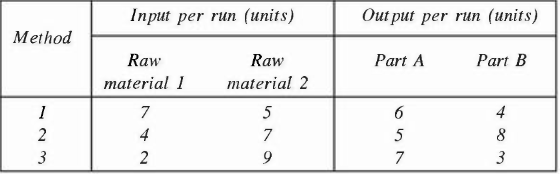
\includegraphics[scale=0.5]{example_production-planning_gupta}
  \scalebox{0.7}{%
    \begin{tabular}{ccccc}
      \toprule
  &\multicolumn{2}{c}{Entrada Por Corrida (unidades)}&\multicolumn{2}{c}{Salidas Por Corrida (unidades)}\\
  \cmidrule{2-5}
  Método&Materia & Materia & Parte&Parte \\
        &prima 1& prima 2&A&B\\
  \midrule
  1&7 &5 &6& 4\\
  2&4&7&5&8\\
  3&2&9&7&3\\
  \bottomrule
\end{tabular}
  } % \scalebox
\par}
\end{frameExample}

\begin{frameExample}{Planeación de la Producción}{}
  La función objetivo a maximizar es  \[ Z = \min \left(  \frac{6x_1 + 5x_2 + 7x_3}{5}, \frac{4x_1 + 8x_2 + 3x_3}{4}\right ) \]
  Las restricciones de disponibilidad de materias primas son:
  \begin{flalign*}
    7x_1 + 4x_2 +2x_3 &\leq 120\\
    5x_1 + 7x_2 +9x_3 &\leq 240\\
  \end{flalign*}
  La formulación anterior viola las propiedades de un programa lineal porque el objetivo es una función no lineal. El modelo se puede transformar a su versión equivalente lineal de la siguiente manera. 
  \[ y =  \min \left(  \frac{6x_1 + 5x_2 + 7x_3}{5}, \frac{4x_1 + 8x_2 + 3x_3}{4}\right )\]
  
\end{frameExample}

\begin{frameExample}{Planeación de la Producción}{}
  Tenemos entonces que
  \begin{flalign*}
    \frac{6x_1 + 5x_2 + 7x_3}{5} & \geq y\\
    \frac{4x_1 + 8x_2 + 3x_3}{4} & \geq y
  \end{flalign*}

  Por lo que el modelo matemático es:
\[ \max Z = y \]
sujeto a (s.t.)
  \begin{columns}[t]
    \column{0.4\textwidth}
\begin{flalign*}
    7x_1 + 4x_2 + 2x_3 & \leq 120\\
    5x_1 + 7x_2 + 9x_3 & \leq 240\\
  \end{flalign*}
  \column{0.4\textwidth}
    \begin{flalign*}
    6x_1 + 5x_2 + 7x_3 - 5y & \geq 0\\
    4x_1 + 8x_2 + 3x_3 - 4y & \geq 0\\
  \end{flalign*}
  \end{columns}
$x_1, x_2, x_3, y   \geq 0 $
\end{frameExample}
%%% Local Variables:
%%% mode: latex
%%% TeX-master: "../slides"
%%% End:



\begin{frameact}{Riser Sports Products}{}
  % Anderson 07-22
  Reiser Sports Products quiere determinar la cantidad de balones de futbol de All-Pro (A)
y Universitario (U) a producir con el fin de maximizar las utilidades durante el siguiente horizonte de planeación de cuatro semanas. Las restricciones que afectan las cantidades de
producción son las capacidades de producción en tres departamentos: corte y teñido, costura
e inspección y empaque. Para el periodo de planeación de cuatro semanas se dispone de 340 horas de corte y teñido, 420 horas de costura y 200 horas de inspección y empaque. Los tiempos requeridos para elaborar un balón A y U en el departamento de corte y teñido son de 12 y 6 horas respectivamente. El departamento de costura requiere 9 horas para un balón A y 6 horas para elaborar un balón U. En la inspección se ocupan 6 horas para cada balón de fútbol. Los balones de futbol All-Pro producen utilidades de \$5 por unidad y los balones Universitarios producen una utilidad de \$4 por unidad. Formule un modelo para el problema.
\end{frameact}



%%% Local Variables:
%%% mode: latex
%%% TeX-master: "../slides"
%%% End:



%%% Local Variables:
%%% mode: latex
%%% TeX-master: "slides_linear-programming-intro"
%%% End:


\begin{frame}
  \maketitle
\end{frame}


\end{document}
